\documentclass[10pt]{article}
\usepackage{microtype,fullpage,graphicx,float}
\title{CS246 Final Project Plan of Attack}
\author{Siddharth Gupta}
\date{Decemeber 2, 2020}
\begin{document}
	\maketitle
	\section{Introduction}
		I am working on the 1-person project ``Straights,'' therefore I will be taking the responsibility of completion for every aspect of this project. As you will see by reading this document, I hope to complete the project well in advance of the deadline with enough time to hopefully complete some extra features.

	\section{Project Breakdown and Timeline}
		\begin{tabular}{|l|l|l|}
				\hline
				\textbf{Item}&\textbf{Start Date}&\textbf{End Date}\\\hline\hline
				Organize project file structure \& make a private Git repo for version control& Dec 1 & Dec 2\\\hline
				Write {\tt main.cc} as a controller and write all header files & Dec 1 & Dec 2\\\hline
				Complete implementation of the project as per the specifications & Dec 3 & Dec 6\\\hline
				Complete thorough testing & Dec 7 & Dec 7\\\hline
				Make fixes based on any errors found during testing & Dec 8 & Dec 8\\\hline
				Finish working on extra features & Dec 9 & Dec 10\\\hline
				Thoroughly test all code: basic \& extra features & Dec 11 & Dec 11\\\hline
				Implement fixes or roll back to previous stable version & Dec 12 & Dec 12\\\hline
				Complete writing of demo plan, design document, and UML & Dec 13 & Dec 14\\\hline
				Submit final code, demo plan, design document, and UML & Dec 15 & Dec 15\\\hline
		\end{tabular}\\\\
		Here, start dates represent the morning of the specified date, while the end date represents midnight. For example, ``Complete thorough testing'' is scheduled to take all of December 7\textsuperscript{th}.
		I expect and will try to match the above mentioned completion dates (or better).

	\section{Responses to Project Specification}
		\begin{figure}[H]
			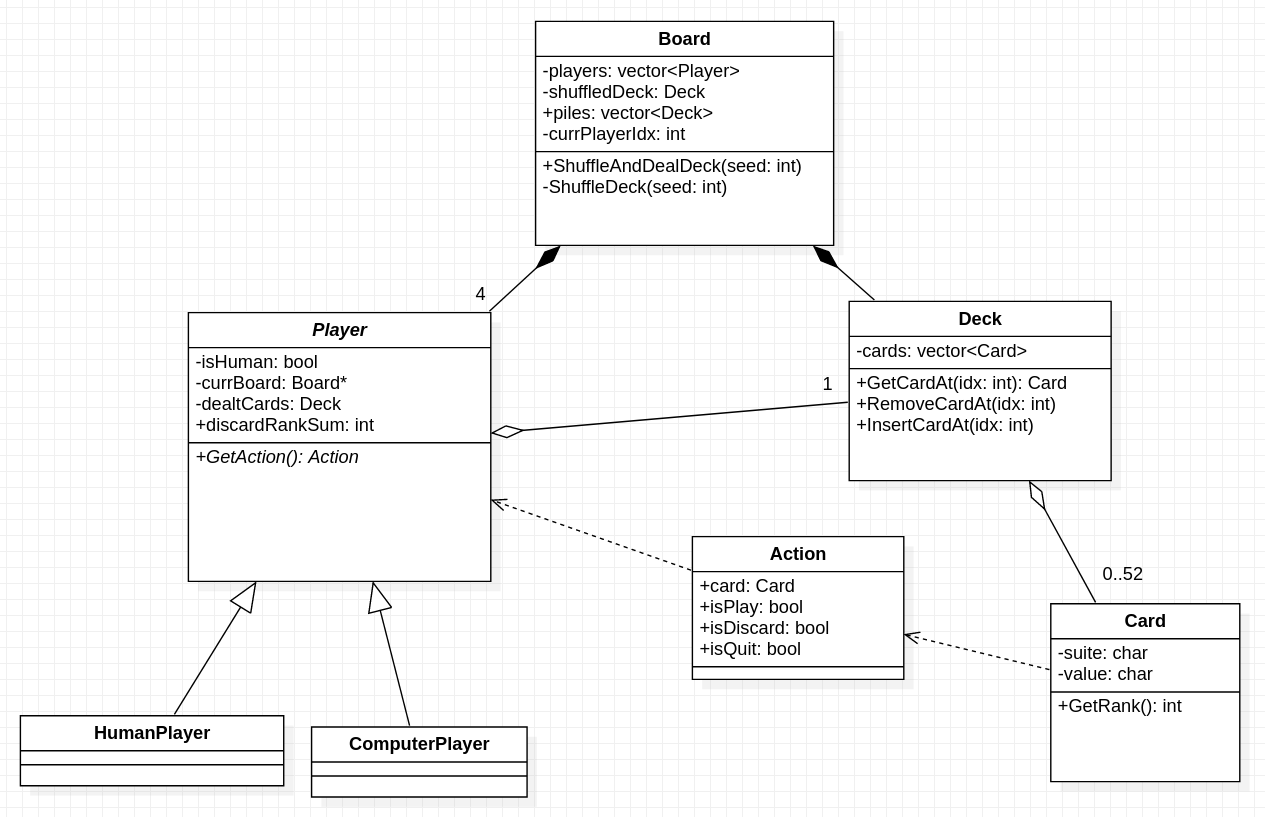
\includegraphics[width=\textwidth]{../uml.png}
			\caption{The anticipated UML diagram representing the project design}
		\end{figure}

		{\bf Question}: What sort of class design or design pattern should you use to structure your game classes so that changing the interface or changing the game rules would have as little impact on the code as possible? Explain how your classes fit this framework.\\
		{\bf Answer}: Since this card game is relatively simple, the majority of game rule handling is being done in the {\tt Board} class, {\tt Player::GetAction} method, and somewhat in {\tt main.cc}. Such a structure allows the ruleset to be broken into parts, handled by the class which it is most related to. For example, if we were to allow cards with rank 6 to be played without a neighbouring ranked card of the same suite (instead of 7), this can become a one-digit change in the implementation of {\tt Player::GetAction}. Since this is expected to be a abstract class, such a change would have to be propagated down to the subclasses, something for which I expect to design a more elegant solution later in this process.
		\\\\
		{\bf Question:} If you want to allow computer players, in addition to human players, how might you structure your classes? Consider that different types of computer players might also have differing play strategies, and that strategies might change as the game progresses i.e.\ dynamically during the play of the game. How would that affect your structure?\\
		{\bf Answer}: Again, referring to the UML diagram, computer players are represented as child classes of a generic {\tt Player} class with a virtual {\tt GetAction} method. This method will be overridden in the implementation of the {\tt ComputerPlayer} class. Since players (both computer and human) have access to the ``board'' through the {\tt currBoard} attribute, they can adapt their logic (i.e.\ strategy) in the {\tt Player::GetAction} method by simply reading the state of the board, allowing for dynamic playstyles during the play of the game.
		\\\\
		{\bf Question}: If a human player wanted to stop playing, but the other players wished to continue, it would be reasonable to replace them with a computer player. How might you structure your classes to allow an easy transfer of the information associated with the human player to the computer player?\\
		{\bf Answer}: In the case where a human player wanted to stop playing while keeping the game running (i.e.\ ragequit), this design allows for a relatively easy switch from a code design perspective. Since any (human) player's state is uniquely identified (relative to other players) by {\tt dealtCards} and {\tt discardRankSum}, that person's {\tt HumanPlayer} object can be deleted and replaced with a {\tt ComputerPlayer} object where the {\tt dealtCards} and {\tt discardRankSum} attributes of the {\tt ComputerPlayer} set to original values (from the human who ``ragequit''). Note, for this player to be ``replaced,'' the change will have to be reflected in {\tt Board::players}, which will eventually be accessible through {\tt Player::currBoard}.
		\\\\

		Note the UML diagram is subject to (and is likely to) change over the course of this project, however the basic design structure and organization is likely to be retained throughout.
\end{document}

